\documentclass{standalone}
\usepackage[T1]{fontenc}
\usepackage[utf8]{inputenc}
\usepackage{sfmath}
\usepackage{tikz}

\begin{document}
\usetikzlibrary{arrows.meta, math}
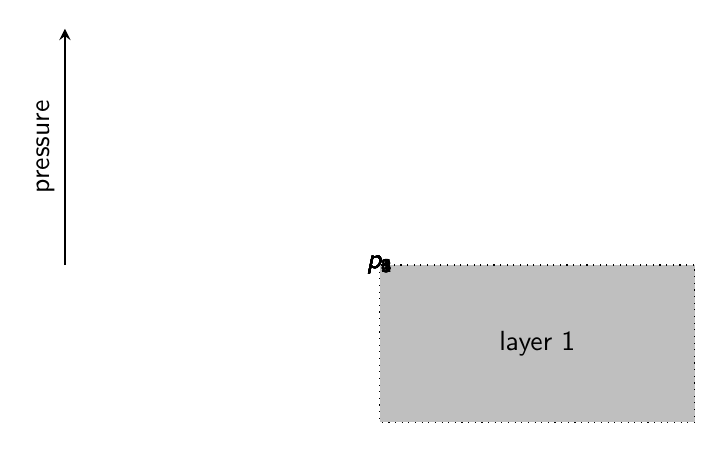
\begin{tikzpicture}[font=\sffamily]

% Draw the left-hand side retrieval grid
\def\Nfirst{4}
\def\Nsecond{3}
\def\Nend{1}
\def\yoffset{0.25}
\def\xoffset{0}
\def\xr{5}

\foreach[count=\i] \y in {\Nfirst,\Nsecond,...,\Nend}
{
    \tikzmath{\yy = \yoffset + \y;}
    \tikzmath{\xx = \xoffset; \xl = \xoffset - 0.5; \xxr = \xoffset + \xr;}

    \ifnum\numexpr\i=1
        \filldraw[draw=black,dotted,fill=lightgray] (\xx,\yy) rectangle (\xr,\yy-1.0) node[pos=.5] {layer 1};
    \fi

    \draw [thick] (\xx,\yy) -- (\xxr,{\yy});
    \node at (\xl,\yy) {$p_{\i}$};
}

% Draw a layer box



% Draw the right-hand side MET grid
\def\Nfirst{5.35}
\def\Nsecond{4.55}
\def\Nend{1.05}
\def\yoffset{-0.5}
\def\xoffset{8}
\def\xr{5}

\foreach[count=\i] \y in {\Nfirst,\Nsecond,...,\Nend}
{
    \tikzmath{\yy = \yoffset + \y;}
    \tikzmath{\xx = \xoffset; \xl = \xoffset - 0.5; \xxr = \xoffset + \xr;}
    \draw [thick] (\xx,\yy) -- (\xxr,{\yy});
    \node at (\xl,\yy) {$p_{\i}$};
}

% Draw the coordinate arrow
\draw [thick, -stealth] (-3,1) -- (-3,4) node [midway, above, sloped] (TextNode) {pressure};


\end{tikzpicture}
\end{document}